\lab{Индукционный газовый разряд}

%Я компилировала файл в Preamble.tex (сбросила его вместе со всеми файлами). При исправлении этой лабы опиралась на работу с магнитометром. Поэтому сейчас в PDF-формате сначала видно 
%Глава 1
%5
%Работа 3.1 (и далее название этой лабы)
%Таким образом, номер главы и номер лабы неверные.

%Также, в работе ниже стоят комментарии около всех формул из теоретического минимума (или введения), который обычно пишется перед лабами с близкими темами. Все номера формул закомментированы и записаны под тем номером, который у них сейчас в лабнике.

%Номер рисунка не читается. В PDF-файле около него стоят ??. Есть комментарий ниже.

%Контрольные вопросы так же стоят после теоретического минимума. В этой лабе и лабе 3.5.2 их не было. Тем не менее, можно в эти лабы добавить вопросы 1, 3--5, 7.

\begin{lab:aim}
{изучение свойств плазмы методом зондовых характеристик.}
\end{lab:aim}

\begin{lab:equipment}{газоразрядная трубка с высокочастотным (ВЧ)-генератором, источник постоянного тока, генератор звуковой частоты
(ЗГ), осциллограф (ЭО), форвакуумный насос, вакуумметр, натекатель, вакуумный кран, делитель (Д), повторители--фазовращатели --- нерегулируемый (ПФ1) и регулируемый (ПФ2).}
\end{lab:equipment}

% Первая строчка ``Оборудования'' каким-то образом в pdf вылезла на поля справа.

Газоразрядную плазму можно получить, используя электрические разряды в переменных высокочастотных (ВЧ) полях. Существуют
различные способы введения ВЧ-поля в разрядный объём. Один из них основан на использовании электромагнитной индукции:
через катушку-соленоид, в которую вставлена диэлектрическая газоразрядная камера, пропускается ток высокой частоты, и
внутри катушки индуцируется вихревое электрическое поле. Силовые линии этого поля, а вместе с~ними линии разрядного
тока, представляют собой замкнутые окружности. Такой разряд называется кольцевым, индукционным или разрядом $H$-типа,
что указывает на определяющую роль магнитного поля. Именно такой способ возбуждения газового разряда используется в нашей
установке.

\experiment
Схема установки представлена на рис. \ref{fig:gazovyj} % номер рисунка не виден после компиляции
. Заполненная газом диэлектрическая камера представляет собой цилиндрическую
стеклянную трубку (ее диаметр и длина указаны в описании), на одном из торцов которой впаяны две молибденовые проволочки (зонды)
диаметром~$d$ и длиной~$l$, расположенные на некотором расстоянии друг от друга. Другой конец трубки не запаян.
Он служит для откачки и для заполнения камеры газом. Трубка вставлена в катушку индуктивности колебательного контура
ВЧ-генератора, работающего на частоте~$\sim10$~МГц. Камера откачивается форвакуумным насосом и с помощью натекателя
заполняется воздухом до давления, указанного в описании работы в лаборатории. Значение давления контролируется вакуумметром
(термопарным манометром).

%\fcpic[1]{5_3_1}{Схема установки для исследования газового разряда}{1}
%\begin{wrapfigure}{r}{0.4\textwidth}
%	\pic{0.38\textwidth}{1_1_1}
%	\caption{Схема установки для исследования газового разряда}
%	\figmark[пфящмно]
%\end{wrapfigure}

\begin{figure}{c}
	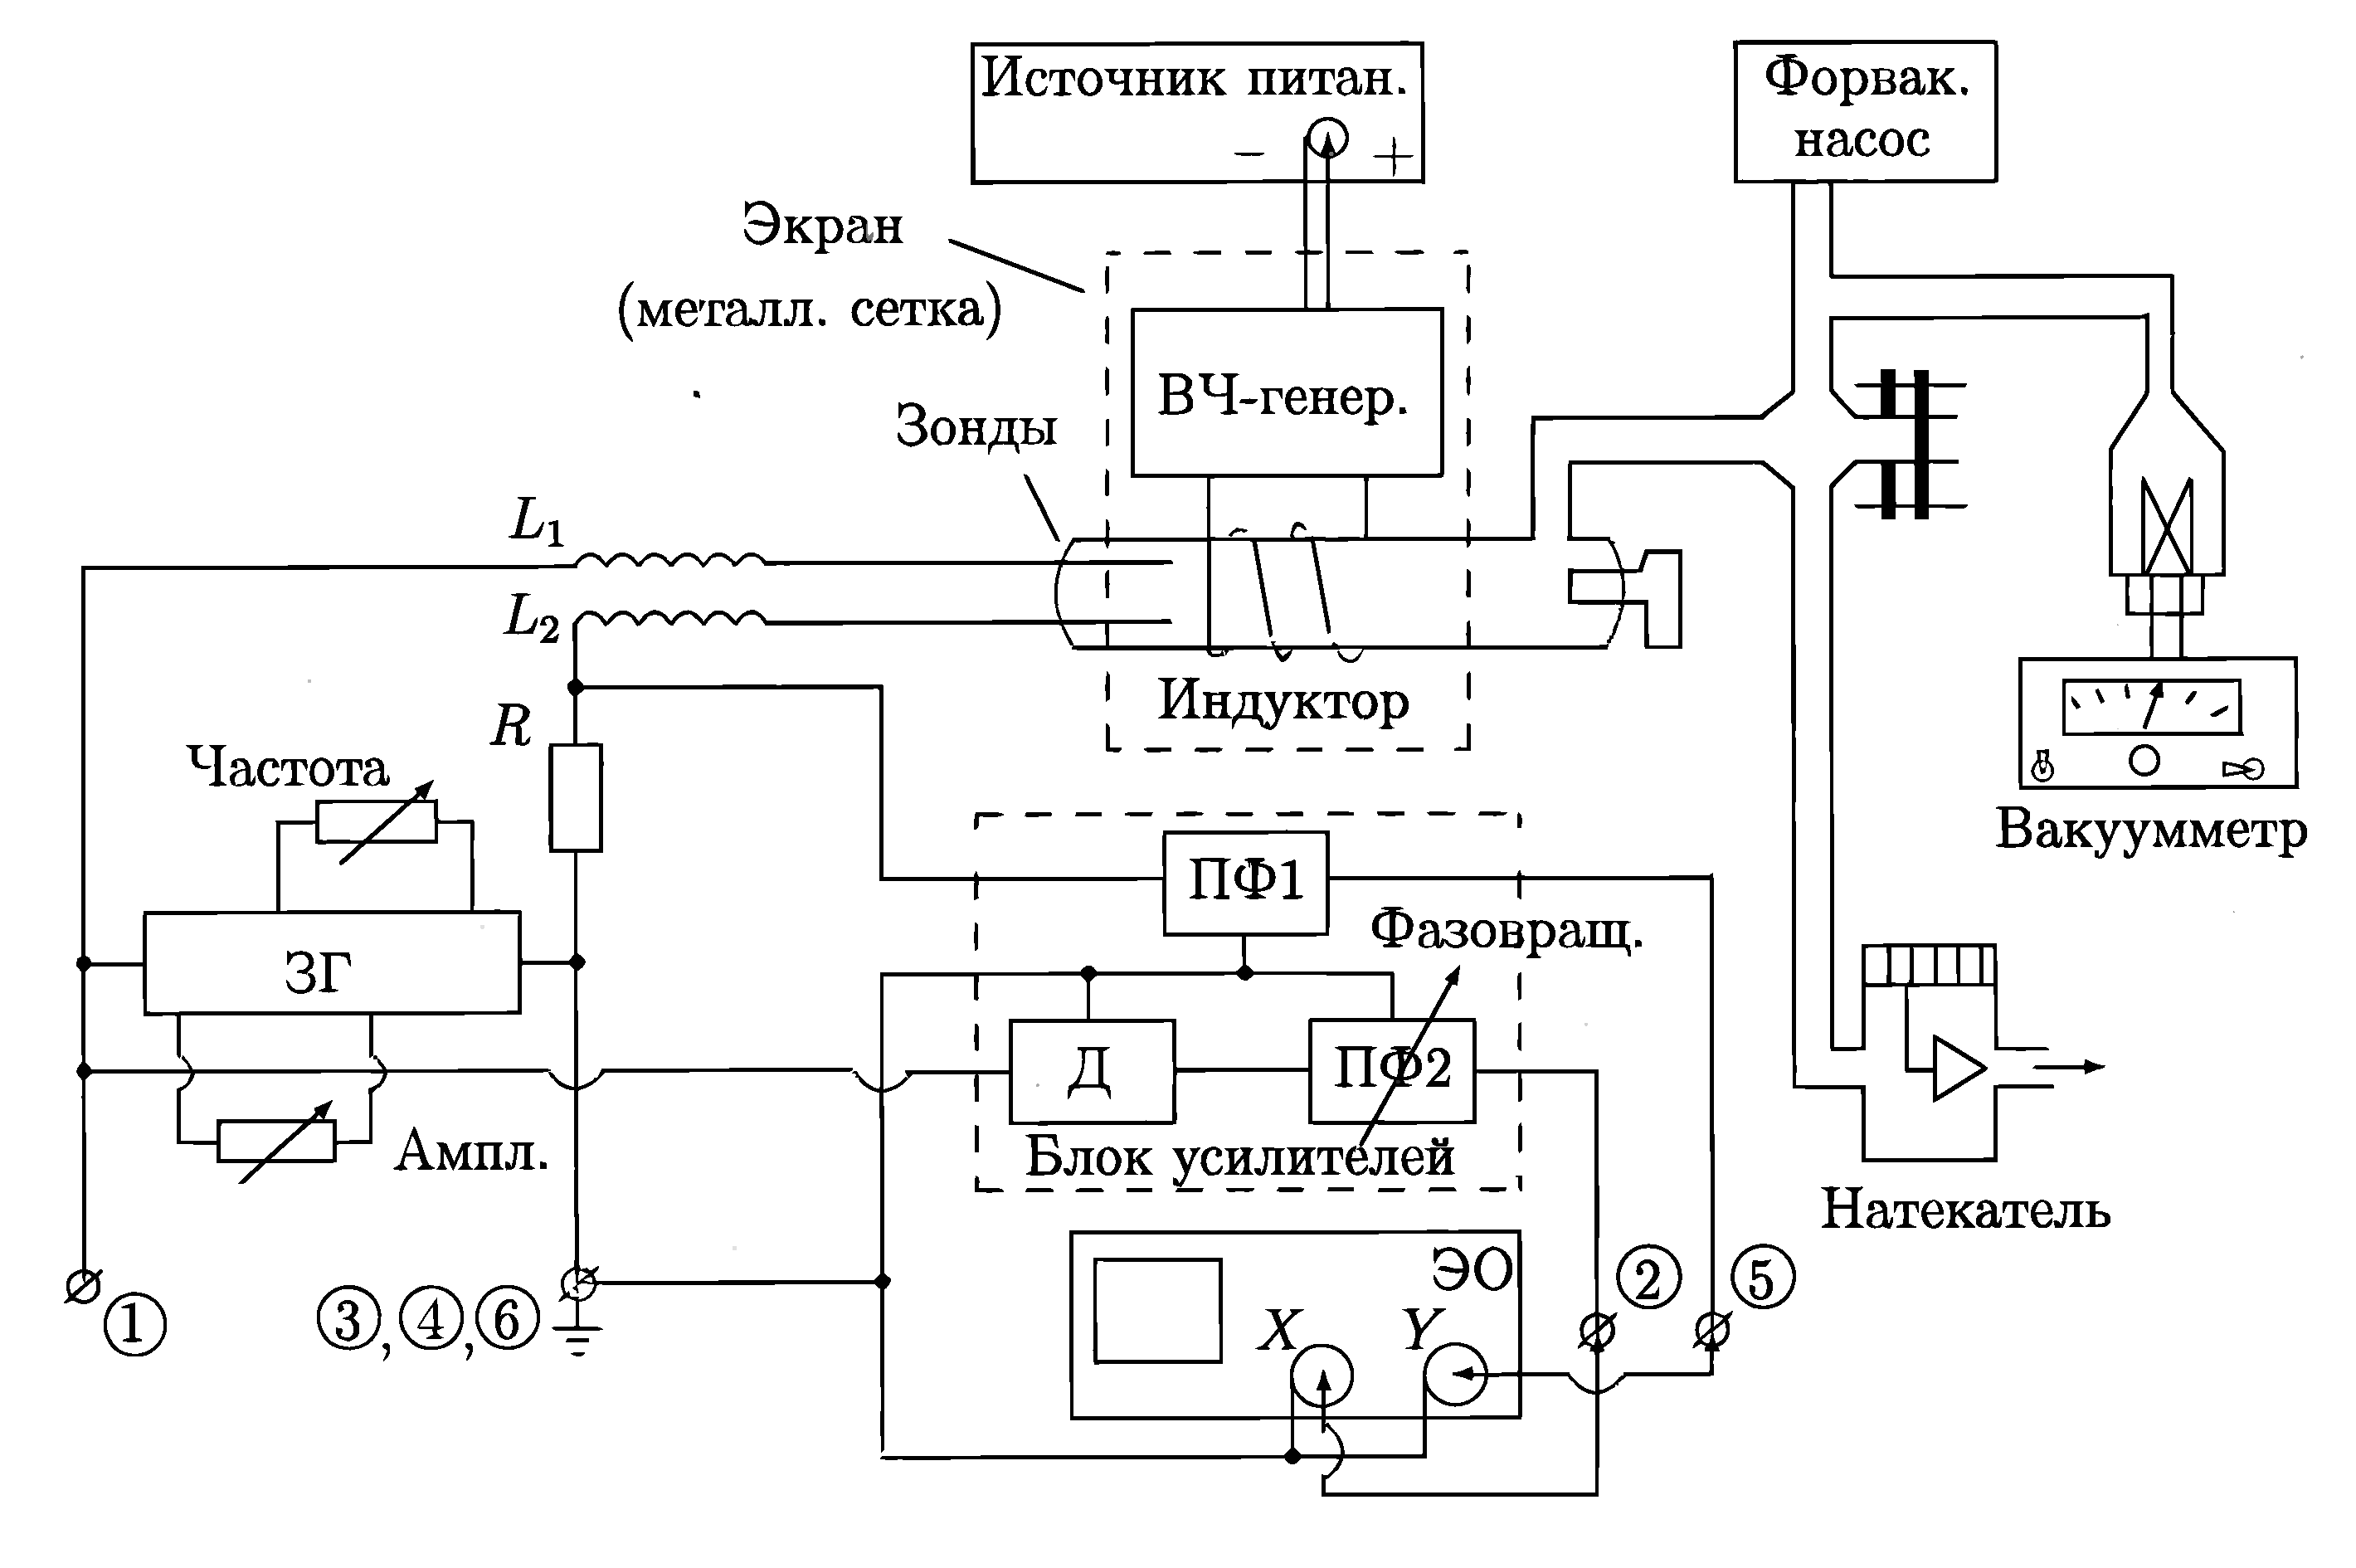
\includegraphics[width=120mm]{Chapter_5/3_5_2.eps}
	\caption{Схема установки для исследования газового разряда}
	\figmark[gazovyj]
\end{figure}

%Когда я компилирую файл с eps, то в левом нижнем углу вылазит буква ``с'' (отдельно от схемы). При просмотре eps и png никакой буквы ``с'' там нет. Появляется только после компиляции.

Следует отметить некоторые особенности процедуры установки рабочего давления в разрядной камере. Установка требуемого давления осуществляется путем изменения проходного сечения натекателя, соединенного с атмосферой, при непрерывной работе откачивающего насоса. При этом скорость откачки сохраняется постоянной, а приток воздуха в разрядную камеру определяется изменением аэродинамического сопротивления нагревателя. Таким образом, устанавливается новое значение давления, при котором скорость откачки насоса уравновешивается расходом воздуха через натекатель.

Изменение сечения натекателя выполняется микрометрическим винтом, который сжимает расположенную под ним пружину и изменяет ее давление на подвижную мембрану клапана. Такая система обладает очень большой инерциальностью и реагирует на вращение винта со значительным запозданием.
 
На зонды поступает синусоидальное напряжение от звукового генератора~ЗГ. Это же напряжение через делитель Д и регулируемый повторитель--фазовращатель ПФ2
подаётся на вход~$X$ осциллографа ЭО. Последовательно с зондом подключен датчик тока - резистор $R$ (значение сопротивления указано в описании работы). Напряжение, пропорциональное току, текущему через плазму, подаётся на вход~$Y$ ЭО через нерегулируемый повторитель-фазовращатель ПФ1. Две катушки $L_{1}$  и $L_{2}$, подключённые к~зондам, не пропускают на осциллограф высокочастотный сигнал. 

На
экране осциллографа наблюдается кривая, представляющая собой вольт-амперную характеристику двойного зонда (см.
рис.~% (5.12) из настоящего лабника \figref{v5_r6}
). Следует отметить, что на некоторых частотах в~измерительной цепи могут возникать фазовые сдвиги, и
характеристика зондов приобретает вид петли. Такие частоты для измерений непригодны. Для устранения фазовых сдвигов используется регулятор фазовращателя ПФ2.  



\begin{lab:task}

В работе предлагается при различных давлениях газа в~трубке получить зондовые вольт-амперные характеристики на экране
осциллографа и рассчитать с~их помощью температуру и~концентрацию электронов в~плазме, степень ионизации, плазменную
частоту и дебаевский радиус экранирования.

\subsection*{Подготовка приборов к работе}

\begin{enumerate}
\item Не включания приборов, ознакомьтесь с установкой (см. описание в лаборатории). 

\item Перед откачкой ознакомьтесь с техническим описанием вакууметра, расположенного на установке, и подготовьте его для работы. Включите форвакуумный насос и вакуумметр. Откачайте трубку до давления, указанного в описании работы в лаборатории. Давление
регулируется с~помощью натекателя (микровентиля) при постоянной откачке.

\item Включите источник питания ВЧ-генератора и проследите за разрядом в трубке: после зажигания разряд должен устойчиво
гореть по всей трубке, включая область расположения зондов.


\item  Включите осциллограф и звуковой генератор, при этом на зонды подается переменное напряжение от ЗГ с частотой, указанной в описании в лаборатории. Подберите напряжение, при котором на экране осциллографа должна появиться кривая, похожая на теоретическую зависимость, изображённую на рис. % рисунок (5.12) настоящего лабника)~\figref{v5_r11}.
Если на кривой не наблюдаются области насыщения, следует увеличить выходное напряжение~ЗГ. Если вместо кривой на экране
возникает петля, ее следует изменить регулировкой фазовращателя.

\item Посмотрите, как ведёт себя разряд, насколько он устойчив при изменении давления в
рабочем диапазоне. Отметьте, в какой области давлений наблюдаемая на экране кривая соответствует
теоретической.
\end{enumerate}

\subsection*{Измерения}

\begin{enumerate}
\item Получите на экране осциллографа вольт-амперную характеристику зондов (см. рис.~%рис.(5.12) настоящего лабника)\eqref{v5_r6}
) для максимального давления из выбранного диапазона.

\item Убедитесь, что ручка плавной регулировки усиления по осям~$X$ и $Y$ выведены вправо до щелчка (при таком положении ручки
чувствительность каналов соответствует величине, указанной возле искретного переключателя усиления). Регулируя напряжение звукового
генератора, добейтесь того, чтобы кривая занимала почти весь экран. При чрезмерно большом напряжении генератора возникает искажение зондовой характеристики, в ее оконечных областях появляются изломы и выпучины. Это происходит вследствие влияния электрического поля зондов на характер плазменного разряда. Такого допускать не следует, уменьшая при необходимости напряжение питания зондов до исчезновения искажений.

\item Зарисуйте кривую с~экрана на кальку. Укажите на
кальке давление (в мВ и м рт.ст.) и чувствительность осциллографа по осям $X$ и $Y$.

\item Повторите измерения п.~6 раздела ``Подготовка приборов к работе'' для 3--4-х давлений внутри интервала, выбранного Вами в п.~5 того же раздела.

\item Закончив работу, выключите сначала насос и немедленно откройте натекатель, затем отключите вакууметр и остальные приборы.

\end{enumerate}

\subsection*{Обработка результатов}

\begin{enumerate}

\item Для каждой кривой пересчитайте масштаб по оси~$Y$ из В/см в А/см, зная сопротивление, с которого сигнал,
пропорциональный зондовому току, подавался на ось~$Y$ осциллографа.

\item Рассчитайте масштаб по оси~$X$ в~В/см с учётом наличия делителя в канале зандового напряжения.

\item По зондовым характеристикам определите температуру~$T_e$ электронов по формуле %(5.43) настоящего лабника \eqref{v5_040}
: ток~$I_{iн}$ %в этом месте буква н в индексе русская, и она не видна после компиляции
найдите
из пересечения асимптоты к~току насыщения с~осью $U=0$ (см. рис.~%(5.12) настоящего лабника \eqref{v5_r11}
); $(dI/dU)|_{u=0}$~--- наклон
характеристики $I=f(U)$ в~точке $U=0$, $I=0$; взяв $\Delta U$ в~вольтах и приняв заряд электрона $e=1$, определите
энергию (<<температуру>>) электронов~$kT_e$ в~электрон-вольтах.

\item Концентрацию электронов $n_e$ определите из формулы (%(5.43) настоящего лабника \eqref{v5_040})\oref{v5_028}
), в которую вместо $n$ следует подставить $n_e$:
\begin{equation}
I_{iн}=0,4n_e eS\sqrt{\frac{2kT_e}{m_i}}.
\end{equation}
Здесь $S=\pi\cdot d\cdot l$~--- площадь поверхности зонда; значения $d$ и $l$ приведены в описании экспериментальной
установки; $m_i=14\cdot 1,66\cdot 10^{-24}$~г~--- масса иона азота.

\item Рассчитайте плазменную частоту колебаний электронов:
\begin{equation}
\omega_p=\sqrt{\frac{n_e e^2}{\epsilon_0 m_e}}.
\end{equation}

\item Рассчитайте дебаевский радиус~$r_{D}$ экранирования по формуле%(5.18) настоящего лабника \eqref{v5_5l})
, которая в случае $T_{e} \gg T_{i}$ принимает вид:
\begin{equation}
r_{D}=\sqrt{\frac{\epsilon_{0}kT_{i}}{n e^{2}}}.
\end{equation}

\item Оцените среднее число ионов в дебаевской сфере по формуле %(5.12) настоящего лабника \eqref{v5_41l})
.

\item Оцените степень ионизации плазмы (долю ионизованных атомов~$\alpha$), если давление в трубке $p \simeq1$~мбар.

\item Оцените погрешности.

\end{enumerate}

\end{lab:task}